\section{Einleitung}
\label{sec:einleitung}

Heutzutage haben Webdienste einen hohen Stellenwert im Internet. Sie sind häufig ein essenzieller Bestandteil von Anwendungen und werden durch eine \textit{Representation State Transfer} (REST)-Schnittstelle für Anwender und Entwickler angeboten. Auch das \textit{Internet of Things} (IoT) bekommt mit fortschreitender Zeit eine immer wichtigere Rolle in der Entwicklung von Anwendungen, wie zum Beispiel in der Hausautomatisierung oder smarte Energieverwaltung, wie in den wissenschaftlichen Berichten \citetitle{HomeAutomationUsingCoAP} von \citeauthor{HomeAutomationUsingCoAP} \autocite{HomeAutomationUsingCoAP}, \citetitle{okur2014study} von \citeauthor{okur2014study} \autocite{okur2014study}, \citetitle{TinyCoAP} von \citeauthor{TinyCoAP} \autocite{TinyCoAP} oder \citetitle{TransportLogisticUsingCoAP} von \citeauthor{TransportLogisticUsingCoAP} \autocite{TransportLogisticUsingCoAP} thematisiert wird.

Um die REST-Architektur auch für eingeschränkte Geräte anbieten zu können, wurde mit \textit{Constrained RESTful Environments} (CoRE) eine geeignete Form geschaffen. Somit können solche Geräte, wie zum Beispiel 8-Bit-Mikrocontroller mit begrenztem Arbeitsspeicher und Readonly-Memory (ROM), als auch Netzwerke, wie zum Beispiel \textit{IPv6 over Low-Power Wireless Area Networks (6LoWPANs)}, solche Architekturen verwenden und realisieren. Damit eine Fragmentierung von Nachrichten in solchen Netzwerken so gering wie möglich auftritt, wird im Constrained Application Protocol (CoAP) ein so niedriger Nachrichten-Overhead wie möglich angestrebt.

Mit CoAP wurde die Entwicklung eines generischen Webprotokolls für die speziellen Anforderungen dieser eingeschränkten Umgebungen, insbesondere mit Hauptaugenmerk auf Energie-, Gebäudeautomatisierungs- und andere Machine-to-Machine (M2M) Anwendungen vorangetrieben. Dabei sollte CoAP keine komprimierte Abwandlung von \textit{Hypertext Transfer Protocol}, abgekürzt HTTP, sein, sondern vielmehr eine Submenge von HTTP mit Verwendung von REST, die für M2M-Szenarien optimiert ist. Somit könnte CoAP leicht dazu verwendet werden, einfache HTTP-Schnittstellen in ein kompaktes Protokoll überzuführen, jedoch bietet CoAP Funktionen an, die speziell in Machine-to-Machine-Anwendungen Verwendung finden. Diese Funktionen sind:
\begin{itemize}
    \item Eingebaute Entdeckung von, im Netzwerk, angebotenen Services und Ressourcen.
    \item Mutlicast-Unterstützung.
    \item Asynchroner Nachrichtenaustausch.
\end{itemize}

In den, von CoAP angedachten Anwendungsgebieten, in denen eine große Menge an Daten über ein Netzwerk fließen, könnten asynchrone Techniken die passende Ergänzung sein, um eine hohe Anzahl von Nachrichten zu empfangen, zu versenden oder zu verarbeiten. Den mit steigender Digitalisierung in privaten als auch geschäftlichem Umfeld, im Form von intelligenter Haussteuerung, effizienter Nutzung von Energieerzeugern und Energieverbrauchern\footnote{\href{https://www.a1energysolutions.at/smartspeicher/}{SmartSpeicher} - intelligente Warmwasserspeicher zur Stabilisierung des Stromnetzes}, steigt auch der Bedarf an leistungsfähigen Anwendungen, die diese schnell anwachsende Anzahl an IoT-Geräten ressourcenschonend und effizient verwalten kann. 

Jedoch eignet sich Asynchronität nicht nur zur Optimierung von Anwendungen im IoT-Bereich, sondern auch für solche mit einer grafischen Programmoberfläche (GUI). Dies hat den Grund, da der für das Zeichnen der Oberfläche verantwortliche Thread freibleibt und somit neu ankommende Eingaben des Benutzers (Mausklick, Tastatureingabe etc.) verarbeiten werden kann, ohne das die Oberfläche "einfriert"\footnote{Beschreibung des Zustandes eines Programmes, indem die Oberfläche keine neuen Eingaben entgegennimmt}.

Dieses Programmierparadigma ist auch nützlich, wenn mit Datenbanken oder REST-Schnittstellen interagiert oder I/O- bzw. CPU-intensive Operationen ausgeführt werden, wie \citeauthor{okur2014study} in deren Studie \citetitle{okur2014study} \autocite{okur2014study} herausgefunden haben.

\subsection{Constrained Application Protocol (CoAP)}
\label{subsec:constrained-application-protocol}

Das \textit{Constrained Application Protocol}, abgekürzt CoAP, ist ein Internetprotokoll, das speziell für M2M Anwendungen, wie zum Beispiel smarte Energieverwaltung oder Hausautomatisierung, entwickelt wurde \autocite{coap}. Dabei bietet das Protokoll ein REST-ähnliches Interface für Mikrocontroller mit angeschlossenen Aktoren oder Sensoren, auch \textit{constrained nodes} genannt, oder auch drahtlose Sensornetze, auch \textit{constrained networks} genannt, an. Die sogenannten \textit{nodes} besitzen meist einen angeschlossenen 8-Bit-Mikrocontroller, der nur eine kleine begrenzte Menge an Arbeitsspeicher (RAM) und Readonly-Memory (ROM) beinhaltet. Bei \textit{contstrained networks}, wie z.B. \textit{IPv6 over Low-Power Wireless Area Networks (6LoWPANs)}, spielt die hohe Paketverlustrate und der für solche Netzwerke typische Datendurchsatz von wenigen 10 kbit/s eine große Rolle. CoAP ist durch den RFC 7252 von \citeauthor{RFC7252} \cite{RFC7252} spezifiziert.

Dabei bietet das \textit{Constrained Application Protocol} ein Interaktionsmodell für Anfragen und Antworten zwischen den, in der Anwendung, definierten Endpunkten an. Auch ist eine eingebaute Entdeckung von, im Netzwerk, angebotenen Services und Ressourcen im Protokoll definiert. Zusätzlich werden Hauptbestandteile des Internets, wie \textit{Unique Resource Identifiers} (URIs) und \textit{Internet Media Types} (zum Beispiel \textit{application/json}) angeboten.

Eine Unterstützung von \textit{Multicast} ist gegeben, als auch ein sehr geringer Mehraufwand in der Datenübertragung. Ferner wurde darauf Wert gelegt, es einfach für eingebettete Systeme zu halten.

Zur Datenübertragung nutzt CoAP das \textit{User Datagram Protocol} (UDP). Dieses unterscheidet sich zum \textit{Transmission Control Protocol} (TCP) in den folgenden Punkten:
\begin{itemize}
    \item Kein Sitzungsaufbau von Sender zu Empfänger (\textit{Handshake}).
    \item Stellt nicht sicher, ob alle Pakete beim Empfänger eintreffen.
    \item Geht ein Paket verloren, wird dieses nicht erneut versendet.
\end{itemize}

Die folgenden Funktionen sind essenzielle Bestandteile von CoAP:
\begin{itemize}
    \item Erfüllung von M2M Anforderungen in eingeschränkten Umgebungen.
    \item UDP-Verbindung mit optionaler Zuverlässigkeit, die Unicast- und Multicast Anfragen unterstützt.
    \item Asynchroner Nachrichtenaustausch.
    \item Niedriger Mehraufwand durch veränderten Header und niedriger Komplexität des Parsings.
    \item URI- und Content-Typen-Support.
    \item Einfache Proxy- und Caching-Unterstützung.
    \item Zustandsloses HTTP-Mapping, welches die Entwicklung von Proxys erlaubt, die den Zugriff auf CoAP Ressourcen über HTTP auf einheitliche Weise ermöglichen oder für einfache HTTP-Schnittstellen, die alternativ über CoAP realisiert werden können.
    \item Sicherheitsmechanismen durch das Anbinden von \textit{Datagram Transport Layer Security} (DTLS).
\end{itemize}

\subsubsection{Begriffe in CoAP}
\label{subsubsec:begiffe-in-coap}

Um den Kontext innerhalb des \textit{Constrained Application Protocols} zu verstehen, werden nachfolgend die wichtigsten Begriffe in CoAP kurz erklärt:
\begin{itemize}
    \item Endpunkt (Endpoint):
          \begin{itemize}
              \item Ein Endpunkt lebt auf einen "Knoten". Ein Knoten ist vergleichbar mit dem Begriff "Host", der vorwiegend in anderen Internetstandards Erwähnung findet.
              \item Ein Endpunkt wird durch Multiplexing-Informationen auf der Transportschicht identifiziert, die eine UDP-Portnummer und eine Sicherheitszuordnung enthalten könnte.
          \end{itemize}
    \item Ursprungsserver (Origin Server):
          \begin{itemize}
              \item Jener Server, auf dem sich eine bestimmte Ressource befindet oder erstellt werden soll.
          \end{itemize}
    \item Bestätigende Nachricht (Confirmable Message):
          \begin{itemize}
              \item Einige Nachrichten benötigen eine Bestätigung des Empfängers. Diese Nachrichten werden als \textit{bestätigt} behandelt.
              \item Falls keine Pakete während der Übertragung verloren gingen, wird für jede Nachricht, die bestätigt werden muss, exakt eine Nachricht des Typs \textit{Acknowledgement} oder \textit{Reset} an den Sender zurückgesendet.
          \end{itemize}
    \item Nicht bestätigende Nachricht (Non-confirmable Message):
          \begin{itemize}
              \item Im Gegensatz zu bestätigenden Nachrichten gibt es auch Nachrichten, die nicht bestätigt werden müssen.
              \item Dies betrifft Nachrichten, die für bestimmte Anwendungsanforderungen häufiger wiederholt werden müssen, wie zum Beispiel, das wiederholte Lesen eines Sensors.
          \end{itemize}
    \item Bestätigungsnachricht (Acknowledgement Message):
          \begin{itemize}
              \item Eine solche Nachricht bestätigt den Empfang einer bestätigenden Nachricht. Eine Bestätigungsnachricht sagt nicht aus, ob die Anfrage, die mit einer bestätigenden Nachricht versendet wurde, erfolgreich war oder nicht.
              \item Jedoch enthält die Bestätigungsnachricht auch eine sogenannte \textit{Piggybacked Response}.
          \end{itemize}
    \item Rücksetzende Nachricht (Reset message):
          \begin{itemize}
              \item Diese Nachricht sagt aus, dass eine spezifische Nachricht, mit dem Typ \textit{Confirmable} oder \textit{Non-confirmable}, empfangen wurde, jedoch einige Teile des Nachrichtenkontextes fehlen, um diese Nachricht korrekt verarbeiten zu können.
              \item Dieses Verhalten tritt auf, wenn der zu empfangende Endpunkt neu gestartet wurde und somit den Zustand vergessen hat, der zur vollständigen Interpretation der Nachricht nötig war.
              \item Ein absichtliches Provozieren einer rücksetzenden Nachricht \textit{Reset Message}, zum Beispiel durch das Senden einer leeren bestätigenden Nachricht (\textit{Empty Confirmable Message}), kann als eine kostengünstige Prüfung der Funktionsfähigkeit eines Endpunktes verwendet werden - vergleichbar mit einem \textit{Ping}.
          \end{itemize}
    \item \textit{"Antwort im Huckepackverfahren"} (Piggybacked Response):
          \begin{itemize}
              \item Eine \textit{Piggybacked Response} ist direkt in eine \textit{Acknowledgement} (ACK) Nachricht inkludiert, die gesendet wird, um den Empfang der Anfrage für diese Antwort zu bestätigen.
          \end{itemize}
    \item Separate Antwort (Separate Response):
          \begin{itemize}
              \item Wenn eine \textit{Confirmable} Nachricht mit einer Anfrage mit einer \textit{Empty} Nachricht quittiert wird (z.B. weil der Server die Antwort nicht sofort hat), wird eine separate Antwort in einem separaten Nachrichtenaustausch gesendet.
          \end{itemize}
    \item Leere Nachricht (Empty Message):
          \begin{itemize}
              \item Eine Nachricht mit dem Code 0.00. Die Nachricht ist weder eine Anfrage noch eine Antwort. Sie beinhaltet nur den 4-Byte-langen Kopf (\textit{header}).
          \end{itemize}
\end{itemize}

\subsubsection{Nachrichtenübertragung}
\label{subsubsec:nachrichtenuebertragung}

CoAP nutzt zur Nachrichtenübertragung UDP, um den Austausch von Nachrichten asynchron ausführen zu können. Dies wird dadurch erreicht, dass eine weitere Schicht auf UDP aufbauend eingefügt wird (siehe Ababbildungung \ref{fig:abstrakte-darstellung-der-verschiedenen-schichten}). Diese Schicht kann optional auch einen Mechanismus zur Sicherstellung des Nachrichtenaustausches beinhalten. Dabei definiert CoAP vier verschiedene Arten von Nachrichten:
\begin{itemize}
    \item Bestätigende Nachricht (\textit{Confirmable Message}),
    \item Nicht bestätigende Nachricht (\textit{Non-confirmable Message}),
    \item Bestätigungsnachricht (\textit{Acknowledgement Message}),
    \item Rücksetzende Nachricht (\textit{Reset Message}),
\end{itemize}

Diese vier Arten stehen orthogonal zueinander, sprich:
\begin{itemize}
    \item Bestätigende und nicht bestätigende Nachrichten sind für Anfragen (\textit{requests}) gedacht.
    \item Rücksetzende Nachrichten oder Nachrichten, die eine Anfrage bestätigen, sind für Antworten (\textit{responses}) gedacht.
\end{itemize}

\begin{figure}[h]
    \centering
    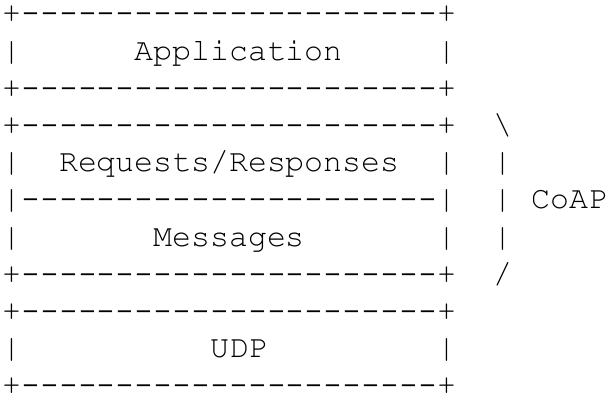
\includegraphics[width=0.5\textwidth]{abstract_layering_of_coap}
    \caption{Abstrakte Darstellung der verschiedenen Schichten (Quelle: RFC 7252 \autocite{RFC7252})}
    \label{fig:abstrakte-darstellung-der-verschiedenen-schichten}
\end{figure}

Das Nachrichtenmodell des Constrained Application Protocols basiert auf den Austausch von Nachrichten über UDP. Dabei beginnt die Nachricht mit einer in der Länge fixierten Vier-Byte-Langen Kopfzeile (\textit{header}), gefolgt von einem optionalen Token (null bis acht Bytes lang), und null oder mehr sogenannten Optionen. Diese Optionen sind vergleichbar mit den \textit{header fields} von HTTP. Nach den Optionen befindet sich ein sogenannter Anhang-Markierer (\textit{Payload marker}), der einem Byte mit acht logischen Einsen, hexadezimal auch 0xFF kodiert, entspricht, jedoch nur in der Nachricht enthalten ist, wenn eine Payload mitgesendet wird. Anschließend an den \textit{Payload marker} kommt der Anhang (\textit{Payload}). Dieses Format ist sowohl für Anfragen als auch für Antworten dasselbe.

Damit Nachrichten als eindeutig identifiziert werden können, wird ein sogenannter Nachrichtenbezeichner (\textit{Message ID}) verwendet. Dieser ist 16 Bit lang und erlaubt somit, bei Implementierungen mit Standardeinstellungen, bis zu 250 Nachrichten die Sekunde von einem Endpunkt zu einem anderen zu senden. Die \textit{Message ID} wird auch für die Sicherstellung des Nachrichtenaustausches (\textit{reliability}) benötigt. Dabei ist jedoch die \textit{Message ID} nur zwischen zwei Endpunkten eindeutig. Kommuniziert ein Teilnehmer mit mehreren Teilnehmern gleichzeitig, dann können die \textit{Message IDs} häufiger vorkommen. Für die eindeutige Identifizierung der Kommunikation zwischen zwei Teilnehmern wird der sogenannte Token verwendet. Dieser ist über mehrere Verbindungen hinweg eindeutig und kann als Identifikator für derzeit laufende Verbindungen gesehen werden.

Die Sicherstellung des Nachrichtenaustausches erfolgt dadurch, dass man eine Nachricht als bestätigend (\textit{Confirmable}) markiert. Eine als \textit{Confirmable} gekennzeichnete Nachricht wird so lange an den jeweiligen Empfänger gesendet, bis dieser eine \textit{Acknowledgement} Nachricht mit derselben \textit{Message ID} zurücksendet (wie in Abbildung \ref{fig:nachrichtenaustausch-mit-sicherstellung-des-transfers} dargestellt). Wenn der Empfänger die \textit{Confirmable} Nachricht, aufgrund fehlender Daten oder fehlendem Kontext nicht beantworten kann, sendet dieser eine \textit{Reset} Nachricht zurück.

\begin{figure}[h]
    \centering
    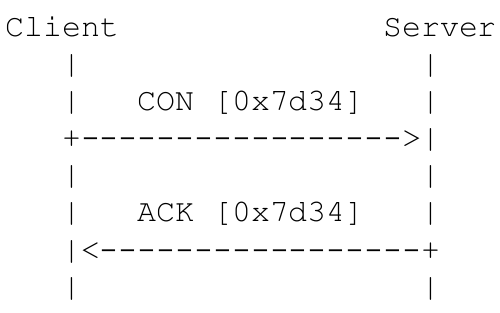
\includegraphics[width=0.5\textwidth]{reliable_message_transmission}
    \caption{Nachrichtenaustausch mit Sicherstellung des Transfers (Quelle: RFC 7252 \autocite{RFC7252})}
    \label{fig:nachrichtenaustausch-mit-sicherstellung-des-transfers}
\end{figure}

Jedoch wird für den Austausch von Nachrichten im CoAP Kontext kein Sicherheitsmechanismus für die Übertragung gefordert, sondern es können auch Nachrichten als \textit{Non-confirmable} markiert werden (siehe Abbildung \ref{fig:nachrichtenaustausch-ohne-sicherstellung-des-transfers}). Diese Vorgangsweise bietet sich zum Beispiel an, wenn man die Messdaten eines Sensors wiederholt ausliest. Dabei werden \textit{Non-confirmable} Nachrichten nicht bestätigt, jedoch wird eine \textit{Message ID} benutzt, um Duplikate zu erkennen.

\begin{figure}[h]
    \centering
    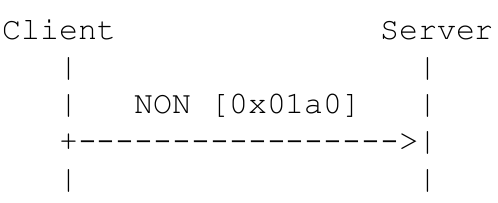
\includegraphics[width=0.5\textwidth]{unreliable_message_transmission}
    \caption{Nachrichtenaustausch ohne Sicherstellung des Transfers (Quelle: RFC 7252 \autocite{RFC7252}).}
    \label{fig:nachrichtenaustausch-ohne-sicherstellung-des-transfers}
\end{figure}

Kann eine ankommende Anfrage (\textit{Request}), welche mithilfe einer \textit{Confirmable} Nachricht versendet wurde, sofort beantwortet werden, wird die Antwort (\textit{Response}) in der daraus resultierenden \textit{Acknowledgment} Nachricht zurückgesendet. Dieses Prinzip nennt man auch \textit{Piggybacked Response}. Das Abbildung \ref{fig:beispiel-eines-erfolgreichen-piggybacked-response} stellt diesen Mechanismus dar.

\begin{figure}[h]
    \centering
    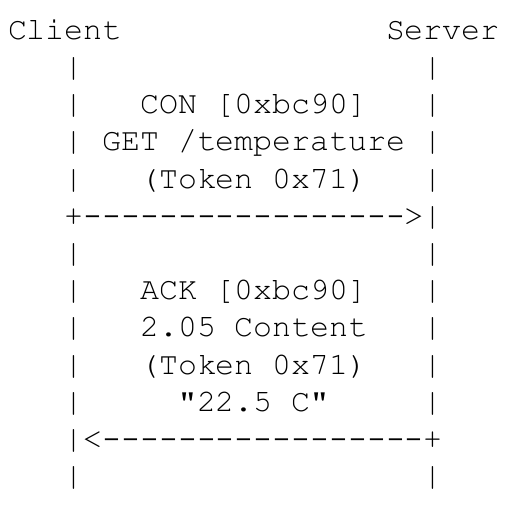
\includegraphics[width=0.5\textwidth]{piggybacked_response}
    \caption{Beispiel einer erfolgreichen \textit{Piggybacked Response} (Quelle: RFC 7252 \cite{RFC7252}).}
    \label{fig:beispiel-eines-erfolgreichen-piggybacked-response}
\end{figure}

Ist der Server jedoch nicht sofort in der Lage die Anfrage zu beantworten, dann antwortet dieser mit einer leeren \textit{Confirmable} Nachricht. Dies macht er, um den Client am wiederholten Senden der Anfrage zu hindern. Sind alle benötigten Daten zur Beantwortung der Anfrage vorhanden, sendet der Server die Antwort in einer neuen \textit{Confirmable} Nachricht zurück. Dieses Prinzip wird als separate Antwort (\textit{separate response}) bezeichnet und wird in der Abbildung \ref{fig:beispiel-einer-separate-response} dargestellt.

\begin{figure}[h]
    \centering
    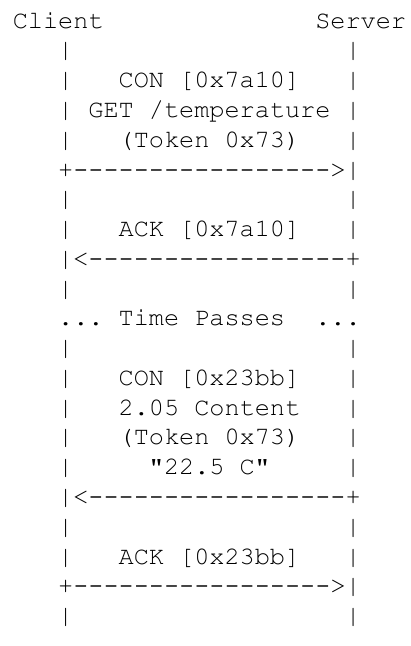
\includegraphics[width=0.5\textwidth]{separate_response}
    \caption{Beispiel einer \textit{separate response} (Quelle: RFC 7252 \cite{RFC7252})}
    \label{fig:beispiel-einer-separate-response}
\end{figure}

Dabei macht CoAP von den bekannten Internetmethoden \textit{GET}, \textit{PUT}, \textit{POST} und \textit{DELETE} in einer ähnlichen Art gebrauch, wie es HTTP macht.

\subsubsection{Nachrichtenformat}
\label{subsubsec:nachrichtenformat}

Wie schon erwähnt, basiert der Nachrichtenaustausch von CoAP auf UDP. Dabei nimmt jede, über UDP versendete Nachricht ein ganzes UDP Datagramm in Anspruch. Der Aufbau einer CoAP Nachricht ist einfach gehalten und startet mit einer Vier-Byte-langen-Kopfzeile (\textit{Header}), welche folgenden Daten beinhaltet, visualisiert in Abbildung \ref{fig:binaere-sturktur-eines-coap-headers}:
\begin{itemize}
    \item \textit{Version}
    \item \textit{Type}
    \item \textit{Token Length}
    \item \textit{Code}
    \item \textit{Message ID}
\end{itemize}

Dabei repräsentieren die ersten zwei Bits des \textit{Headers} die Versionsnummer. Die Versionsnummer gibt an, in welcher CoAP Version die Nachricht erstellt wurde bzw. verarbeitet werden kann. In dieser Arbeit beschäftigen wir uns mit CoAP Nachrichten mit der Versionsnummer 1, in Binär als 01 kodiert.

Die darauffolgenden zwei Bits entsprechen dem Typ der CoAP Nachricht. Der Typ gibt an, ob es sich um eine \textit{Confirmable} (0 = in Binär als 00 kodiert), \textit{Non-Confirmable} (1 = 01), \textit{Acknowledgement}  (2 = 10) oder \textit{Reset} (3 = 11) Nachricht handelt.

Als Nächstes kommt die vier Bit lange \textit{Token Length}, welche die Länge des \textit{Tokens} angibt. Dabei kann der \textit{Token} zwischen null, in Binär als 0000 kodiert, und acht, in Binär als 0111 kodiert, Bytes lang sein. \textit{Token Lengths}, welche zwischen neun und fünfzehn Bytes lang sind, sind im RFC 7252 \autocite{RFC7252} für zukünftige Versionen reserviert.

Die nächsten acht Bit geben den \textit{Code}, vergleichbar mit dem Statuscode bei HTTP, der CoAP Nachricht an. Dabei unterteilt sich der \textit{Code} in eine drei Bit lange \textit{Code Class} (\textit{most significant bits}) und einen fünf Bit langen \textit{Code Detail} (\textit{least significatn bits}). Dabei folgt der \textit{Code} dem Schema "c.dd", wobei "c" Werte von 0 bis 7 annehmen kann und "dd" Werte von 00 bis 31. Die \textit{Code Class} gibt dabei an, ob es sich um
\begin{itemize}
    \item eine Anfrage (0),
    \item eine erfolgreiche Antwort (2),
    \item eine clientseitige, fehlerhafte Antwort (4),
    \item oder eine serverseitige, fehlerhafte Antwort (5) handelt.
\end{itemize}

Daneben nimmt der \textit{Code} 0.00 eine besondere Stellung ein, da dieser eine leere Nachricht (\textit{Empty Message}) markiert. Die \textit{Codes} gleichen sich mit einigen Statuscodes, welche man von HTTP kennt, jedoch ist nicht jeder Statuscode als CoAP \textit{Code} abgebildet.

Der letzte Teil des \textit{Headers} ist die sogenannte \textit{Message Id}, die 16 Bit in Anspruch nimmt und in der \textit{Network Byte Order}, auch unter dem Begriff \textit{Big Endian} bekannt, angegeben wird. Dessen Aufgabe ist es, Duplikate von Nachrichten zu erkennen. Auch wird die \textit{Message Id} dafür benutzt, um Nachrichten vom Typ \textit{Acknowledgement} und \textit{Reset} zu Nachrichten vom Typ \textit{Confirmable} und \textit{Non-Confirmable} zu verlinken. Somit besitzt der Server immer einen Überblick, zu welcher Anfrage schon eine Antwort geschickt wurde.

\begin{figure}[h]
    \centering
    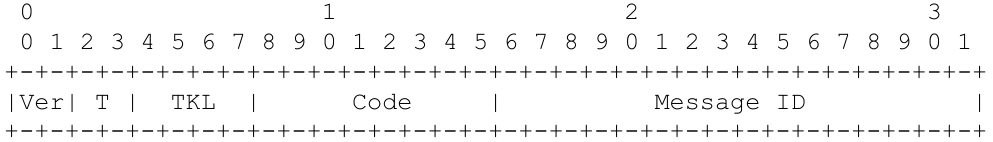
\includegraphics[width=0.75\textwidth]{coap_header}
    \caption{Binäre Struktur eines CoAP \textit{Headers} (Quelle: RFC 7252 \autocite{RFC7252})}
    \label{fig:binaere-sturktur-eines-coap-headers}
\end{figure}

Anschließend an den \textit{Header} kommt der \textit{Token} der Nachricht. Dieser ist in seiner Länge variabel und hängt von der im \textit{Header} angegebenen \textit{Token Length} ab. Dieser ist zuständig für die Korrelation von Anfragen zu Antworten.

Nachfolgend können null oder mehr sogenannte \textit{Options} folgen. Der Option können folgende Bestandteile einer CoAP Nachricht folgen:
\begin{itemize}
    \item Das Ende der CoAP Nachricht (EoF),
    \item Eine weitere Option,
    \item Oder der \textit{Payload Marker} mit anschließender \textit{Payload}.
\end{itemize}

Ist eine \textit{Payload} gegeben, folgt nach der Gruppe von Optionen ein sogenannter \textit{Payload Marker}. Dieser besteht aus einem Byte voller logischer Einsen, hexadezimal als 0xFF kodiert, und markiert somit das Ende der \textit{Options}. Alle Daten, die sich nach dem \textit{Payload Marker} befinden, werden als \textit{Payload} interpretiert. Dabei ist die Länge durch die \textit{UDP Datagram} Paketgröße von 65 535 Bytes begrenzt. Werden für die Übertragung der Nachricht mehr Bytes benötigt als ein \textit{UDP Datagram} an Größe bereitstellen kann, werden die Bytes auf mehrere \textit{UDP Datagrams} aufgeteilt. Diesen Mechanismus nennt man auch \textit{Blockwise transfer} und wird im RFC 7959 von \citeauthor{RFC7959} \cite{RFC7959}, der auf dem RFC 7252 von \citeauthor{RFC7252} \autocite{RFC7252} aufbaut, beschrieben.

\begin{figure}[h]
    \centering
    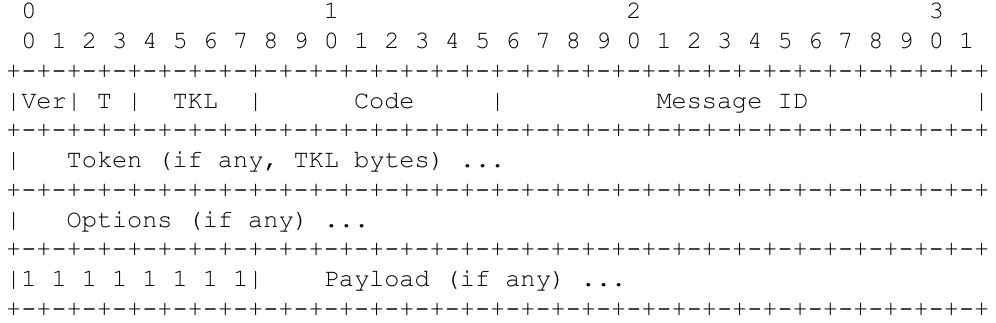
\includegraphics[width=0.75\textwidth]{coap_message}
    \caption{Binäre Struktur einer vollständigen CoAP Nachricht (Quelle: RFC 7252 \autocite{RFC7252})}
    \label{fig:binaere-sturktur-einer-vollstaendigen-coap-nachricht}
\end{figure}

\subsubsection{Aufbau einer Option}
\label{subsubsec:aufbau-einer-option}

Eine Option wird durch eine eindeutige Nummer identifiziert. Neben der Nummer besitzt eine Option auch einen Wert (\textit{Value}), den diese Option hält, und einen Indikator für die Länge des Wertes. Dabei wird die Nummer nicht direkt in die Nachricht kodiert, sondern die Optionen werden zuerst aufsteigend nach ihrer Nummer sortiert und dann wird eine Deltakodierung (Differenzbildung) zwischen der aktuellen Option und deren Vorgängern gebildet. Dies geschieht dadurch, dass alle vorherigen Differenzen, auch im RFC 7252 \autocite{RFC7252} als \textit{Delta} bezeichnet, addiert werden und dann die Differenz zur aktuellen Option gebildet wird. Für die erste Option wird der Sonderfall behandelt, dass als vorheriges Delta ein Wert von null angenommen wird. Dies resultiert daraus, dass für die erste Option die kodierte Differenz als Nummer der Option verwendet wird. Ein weiterer Sonderfall ist derjenige, wenn mehrere Instanzen der gleichen Option in der Kollektion von Optionen auftritt. Dabei ist die Differenz zwischen zwei gleichen Optionen immer null.

Eine Option fängt immer mit einem Byte an, das zwei Informationen enthält. Einmal die Differenz (\textit{Option Delta}) und andererseits die Länge des Wertes (\textit{Option Length}) der Option. Das \textit{Option Delta} entspricht dabei den ersten vier Bits (\textit{most significant bits}) und die \textit{Option Length} den letzten vier Bits (\textit{least significant bits}). Man kann dieses Byte auch als einen \textit{Header} für Options bezeichnen, da dieser Informationen beinhaltet, die für das Kodierung bzw. Dekodieren von Options benötigt wird.

Um jedoch Deltas und Längen, jenseits des Wertes fünfzehn, verwenden zu können, können dem \textit{Option Header} das \textit{Option Delta (extended)} und die \textit{Option Length (extended)} folgen. Diese beiden können jeweils zwischen null und zwei Bytes lang sein. Nach diesen beiden folgt der sogenannte \textit{Option Value}, der null oder mehr Bytes betragen kann.

\begin{figure}[h]
    \centering
    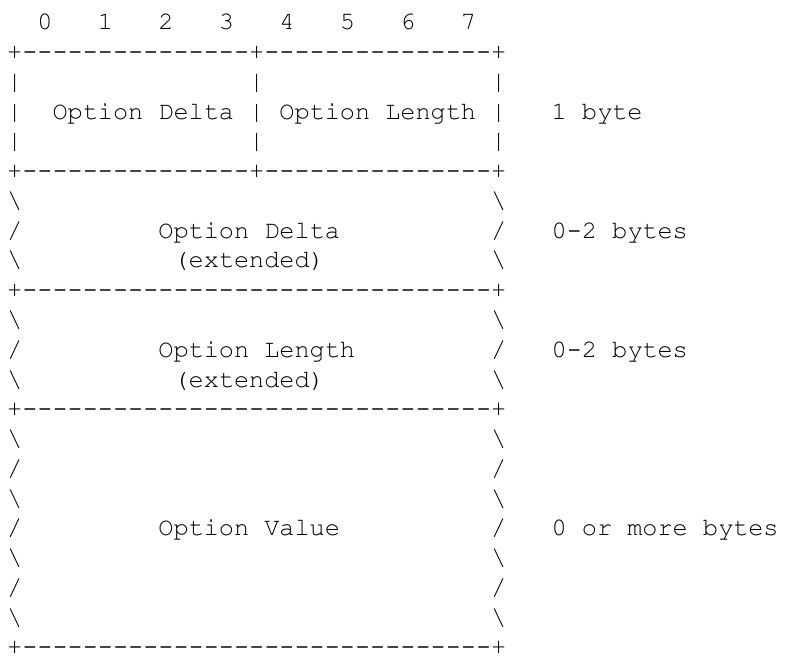
\includegraphics[width=0.75\textwidth]{structure_option.png}
    \caption{Binäre Struktur einer CoAP-Option (Quelle: RFC 7252 \autocite{RFC7252})}
    \label{fig:binaere-sturktur-einer-coap-option}
\end{figure}

\subsection{Ausführungsparadigmen in der Informatik}
\label{subsubsec:ausfuehrungsparadigmen-in-der-informatik}

In der Informatik spricht man von zwei großen Ausführungsparadigmen, mit denen Programme bzw. Codeteile ausgeführt werden können: \textbf{synchrone} und \textbf{asynchrone Ausführung}. Diese beiden Ausführungsparadigmen unterscheiden sich in wesentlichen Punkten deutlich voneinander und bieten in verschiedenen Einsatzszenarien Vor- und Nachteile (siehe Tabelle \ref{tab:vergleich-synchroner-asynchroner-Ausfuehrung}). Dabei unterstützen die geläufigsten Programmiersprachen von Haus aus eine synchrone Ausführung von Programmen, jedoch bieten nicht alle eine asynchrone Ausführung.

\begin{table}[h]
    \resizebox{\textwidth}{!}{%
        \begin{tabular}{@{}lll@{}}
            \toprule
                          & Synchron                                       & Asynchron                                       \\ \midrule
            Programmfluss & Stoppt den Programmfluss.                      & Kann im Programmfluss weiter gehen.             \\ \midrule
            Beendigung    & Überprüft periodisch, ob Funktion beendet ist. & Ein Event markiert die Beendigung der Funktion. \\ \midrule
            Main-Thread   & Ist als "Blocked" oder "Waiting" markiert.     & Ist frei für andere Aufgaben.                   \\ \bottomrule
        \end{tabular}%
    }
    \caption{Vergleich zwischen synchroner und asynchroner Ausführung}
    \label{tab:vergleich-synchroner-asynchroner-Ausfuehrung}
\end{table}

Um diese Unterschiede zwischen den beiden Paradigmen zu veranschaulichen, wird dies anhand einer Client-Server-Anwendung mit einer an den Server angeschlossenen Datenbank und zwei Clients verbildlicht (siehe Abbildungen \ref{figure:sequendiagramm-eines-synchronen-servers} und \ref{figure:sequendiagramm-eines-asynchronen-servers}). Dabei ist der Server eine einfache Web-Applikation, welcher die Daten mittels SQL von der angeschlossenen Datenbank holt.

Senden nun beide Clients, in kurzem Zeitabstand zueinander, eine Anfrage an den Server, so kann der synchrone Server nur die Anfrage bearbeiten, die zuerst eintrifft - in diesem Fall die des Client 1. Dies geschieht deswegen, da der Main-Thread bzw. der für das Empfangen der Pakete zuständige Thread auf die Rückantwort des Datenbankservers wartet. Dadurch wird die Anfrage von Client 2 auf dem Server zurückgehalten und erst bearbeitet, wenn die erste Anfrage bearbeitet und zurückgesendet wurde. Dieses Verhalten skaliert schlecht mit mehreren, gleichzeitig eintreffenden Anfragen, da der sogenannte \textit{Threadpool}\footnote{Entspricht einer Queue in der die zu bearbeitenden Aufgaben abgelegt werden.}, bei zu vielen, langandauernden Anfragen, seine Kapazitätsgrenze erreicht und somit keine neuen Anfragen / Aufgaben annehmen kann.

\begin{figure}[ht]
    \centering
    \begin{tikzpicture}
        \node at (0,.3) {Database};
        \node at (-3,.3) {Server};
        \node at (-6,.3) {Client 2};
        \node at (-9,.3) {Client 1};

        \draw[thick, uibkorange] (-9,0) -- node[left] {prepare}(-9,-0.5);
        \draw[thick, uibkgraym] (-6,0) -- (-6,-0.5);
        \draw[thick, uibkgraym] (-3,0) -- (-3,-0.5);
        \draw[thick, uibkgraym] (-0,0) -- (0,-0.5);
        \draw[->, thick, uibkorange] (-9,-0.5) -- node[midway,above] {Request 1} (-3,-0.5);
        \draw[thick, uibkorange] (-3,-0.5) -- node[left] {prepare SQL}(-3,-1);
        \draw[->, thick, uibkorange] (-3,-1) -- node[midway,above] {SQL Request 1} (-0,-1);
        \draw[thick, uibkgraym] (0, -0.5) -- (0, -1);
        \draw[thick, uibkorange] (-0,-1) -- node [right] {execute} (0,-3);
        \draw[thick, uibkgraym] (-6, -0.5) -- (-6, -1);
        \draw[thick, uibkblue] (-6, -1) -- node[left] {prepare} (-6, -1.5);
        \draw[->, thick, uibkblue] (-6,-1.5) -- node[midway,above] {Request 2} (-3,-1.5);
        \draw[thick, uibkgraym] (-3,-1) -- (-3,-1.5);
        \draw[<-, thick, uibkorange] (-3,-3) -- node [midway, above] {SQL Response 1} (0,-3);
        \draw[thick, uibkgraym] (-3,-1.5) -- (-3,-3);
        \draw[thick, uibkorange] (-3,-3) -- (-3,-3.5);
        \draw[<-, thick, uibkorange] (-9,-3.5) -- node [midway, above] {Response 1} (-3,-3.5);
        \draw[thick, uibkgraym] (-9,-0.5) -- (-9,-3.5);
        \draw[thick, uibkorange] (-9,-3.5) -- node [midway, left] {process} (-9,-5.5);
        \draw[thick, uibkblue] (-3,-3.5) -- node [midway, left] {prepare SQL} (-3,-4);
        \draw[thick, uibkgraym] (-0,-3) -- (-0,-4);
        \draw[->, thick, uibkblue] (-3,-4) -- node [midway, above] {SQL Request 2} (-0,-4);
        \draw[thick, uibkblue] (-0,-4) -- node [midway, right] {execute} (-0,-5);
        \draw[thick, uibkgraym] (-3,-4) -- (-3,-5);
        \draw[<-, thick, uibkblue] (-3,-5) -- node [midway, above] {SQL Response 2} (-0,-5);
        \draw[thick, uibkblue] (-3,-5) -- (-3,-5.5);
        \draw[thick, uibkgraym] (-6,-1.5) -- (-6,-5.5);
        \draw[<-, thick, uibkblue] (-6,-5.5) -- node [midway, above] {Response 2} (-3,-5.5);
        \draw[thick, uibkgraym] (0, -5) -- (0, -5.5);
    \end{tikzpicture}
    \caption{Sequenzdiagramm eines synchronen Servers}
    \label{figure:sequendiagramm-eines-synchronen-servers}
\end{figure}

Setzt man anstelle eines synchronen Servers einen asynchronen Server ein, so ändert sich das beschriebene Szenario folgendermaßen: Trifft die Anfrage des Client 1 ein, wird diese, wie zuvor, sofort abgearbeitet. Dies geschieht jedoch auf einen anderen Thread, damit der Main-Thread bzw. der für das Empfangen der Pakete zuständige Thread wieder frei wird. Wird nun vom Client 2 eine Anfrage verschickt, dann kann der Server diese entgegennehmen und auf einen weiteren, freien Thread verlagern und bearbeiten. Je nachdem welche Anfrage schneller vom Datenbankserver verarbeitet wird, in diesem Fall die des Client 1, wird der Main-Thread bzw. der Thread, der das Paket zuvor entgegengenommen hat, über die Beendigung der Datenbankanfrage benachrichtigt. Somit kann dieser Thread seinen Kontext synchronisieren und die Antwort an den Client 1 zurücksenden.

Dieses Verfahren skaliert deutlich besser mit steigender Anzahl von Anfragen, jedoch kann dies auch mehr CPU- und Speicherressourcen verursachen. Dies liegt daran, dass zum Aufrechterhalten des Zustandes eine asynchrone Zustandsmaschine konstruiert wird und der Kontextwechsel bei Beendigung des asynchronen Aufrufs mit den Main-Thread synchronisiert werden muss.

\begin{figure}[ht]
    \centering
    \begin{tikzpicture}
        \node at (0,.3) {Database};
        \node at (-3,.3) {Server};
        \node at (-6,.3) {Client 2};
        \node at (-9,.3) {Client 1};
        
        \draw[thick, uibkorange] (-9,0) -- node[left] {prepare}(-9,-0.5);
        \draw[thick, uibkgraym] (-6,0) -- (-6,-0.5);
        \draw[thick, uibkgraym] (-3,0) -- (-3,-0.5);
        \draw[thick, uibkgraym] (-0,0) -- (0,-0.5);
        \draw[->, thick, uibkorange] (-9,-0.5) -- node[midway,above] {Request 1} (-3,-0.5);
        \draw[thick, uibkorange] (-3,-0.5) -- node[left] {prepare SQL}(-3,-1);
        \draw[thick, uibkgraym] (-6,-0.5) -- (-6,-1.5);
        \draw[->, thick, uibkorange] (-3,-1) -- node[midway,above] {SQL Request 1} (-0,-1);
        \draw[thick, uibkgraym] (0, -0.5) -- (0, -1);
        \draw[thick, uibkorange] (-0,-1) -- node [right] {execute} (0,-3);
        \draw[thick, uibkgraym] (-3,-1) -- (-3,-1.5);
        \draw[->, thick, uibkblue] (-6,-1.5) -- node[midway,above] {Request 2} (-3,-1.5);
        \draw[thick, uibkblue] (-3,-1.5) -- node[midway, left] {prepare SQL} (-3,-2);
        \draw[->, thick, uibkblue] (-3,-2) -- node [midway, above] {SQL Request 2} (-0,-2);
        \draw[thick, uibkgraym] (-3,-2) -- (-3,-3);
        \draw[<-, thick, uibkorange] (-3,-3) -- node [midway, above] {SQL Response 1} (0,-3);
        \draw[thick, uibkorange] (-3,-3) -- (-3,-3.5);
        \draw[<-, thick, uibkorange] (-9,-3.5) -- node [midway, above] {Response 1} (-3,-3.5);
        \draw[thick, uibkgraym] (-9,-0.5) -- (-9,-3.5);
        \draw[thick, uibkblue] (-0,-3) -- node [midway, right] {execute} (-0,-4);
        \draw[thick, uibkorange] (-9,-3.5) -- node [midway, left] {process} (-9,-5.5);
        \draw[thick, uibkgraym] (-3,-3.5) -- (-3,-4);
        \draw[<-, thick, uibkblue] (-3,-4) -- node [midway, above] {SQL Response 2} (-0,-4);
        \draw[thick, uibkblue] (-3,-4) -- (-3,-4.5);
        \draw[thick, uibkgraym] (0,-4) -- (0,-5.5);
        \draw[<-, thick, uibkblue] (-6,-4.5) -- node [midway, above] {Response 2} (-3,-4.5);
        \draw[thick, uibkgraym] (-6,-1.5) -- (-6,-4.5);
        \draw[thick, uibkblue] (-6,-4.5) -- node [midway, left] {process} (-6,-5.5);
        \draw[thick, uibkgraym] (-3,-4.5) -- (-3,-5.5);
    \end{tikzpicture}
    \caption{Sequenzdiagramm eines asynchronen Servers}
    \label{figure:sequendiagramm-eines-asynchronen-servers}
\end{figure}

\subsubsection{Asynchronität in C\#}
\label{subsubsec:ansynchronitaet-in-csharp}

Mit \textit{Task-based Asynchronous Pattern} (TAP) ermöglicht Microsoft in C\# Asynchronität. Dieses Pattern ermöglicht eine einfache Transformation von synchronen Code zu asynchronen Code ohne große Änderungen vornehmen zu müssen. Auch ist es von Haus aus im Sprachkonstrukt von C\# integriert und kann somit ohne zusätzliche Konfiguration verwendet werden.

Dabei baut das asynchrone Ausführungsparadigma für C\# auf folgende Komponenten auf:
\begin{itemize}
    \item \mintinline{csharp}{Task}: Ermöglicht eine asynchrone Methode zu definieren.
    \item \mintinline{csharp}{Task<TResult>}: Ermöglicht einen Rückgabewert vom Typ TResult von einer asynchronen Methode zurückzugeben.
    \item \mintinline{csharp}{CancellationToken}: Ermöglicht es einen Aufruf einer asynchronen Methode vorzeitig zu beenden.
    \item \mintinline{csharp}{async}/\mintinline{csharp}{await}: Schlüsselwörter um asynchrone Methoden zu deklarieren und auszuführen.
\end{itemize}

Im nachfolgenden Listing \ref{listing:synchrone-methode-in-csharp} wird eine Instanz eines DownloadClient erzeugt. Dieser besitzt eine Methode \textit{Download}, mit welcher der Inhalt einer Webseite heruntergeladen und als \mintinline{csharp}{string} zurückgegeben werden kann.

\begin{listing}[H]
    \inputminted[framesep=2mm, baselinestretch=1.2, fontsize=\normalsize, linenos]{csharp}{codes/example_synchronous.cs}
    \caption{Synchrone Methode in C\#}
    \label{listing:synchrone-methode-in-csharp}
\end{listing}

Diese Vorgehensweise hat den Nachteil, dass die Funktion den Main-Thread bzw. den Thread, der diese Methode aufgerufen hat, solange blockiert bis der gesamte Webseiteninhalt der angegebenen URI heruntergeladen wurde. Bei UI-Anwendungen lässt sich dadurch die Oberfläche nicht mehr bedienen und friert ein. Bei Verwendung in einer Konsolen-Applikation ohne UI ist der Main-Thread bis auf Weiteres blockiert und somit können andere Programmteile, die nicht auf das Ergebnis dieser Methode angewiesen sind, nicht ausgeführt werden.

Damit der aufzurufende Thread bzw. der Main-Thread nicht andauernd auf die Beendigung der Methode warten muss, kann man Events einsetzen, wie in Listing \ref{listing:eventbasierte-methode-in-csharp} dargestellt. Diese beendigen vorzeitig die Exekution der Methode, indem der Aufrufer ein Objekt übergeben bekommt. Dieses Objekt repräsentiert den derzeitigen Zustand der Operation - also in diesem Fall das Herunterladen des Webseiteninhaltes. Dafür wird in Zeile 3 das \mintinline{csharp}{DownloadResult}-Objekt erzeugt. In Zeile 5 wird durch den Operator \mintinline{csharp}{+=} die nachfolgende anonyme Lambdafunktion \mintinline{csharp}{(content) => result.SetComplete(content)} als Beobachter des Events \mintinline{csharp}{client.DownloadComplete} registriert. Diese Lambdafunktion hat die Aufgabe den heruntergeladen Inhalt der Webseite in das DownloadResult zu setzen und als vollständig zu markieren. Dies passiert durch den Aufruf der Methode \mintinline{csharp}{SetComplete(string content)} auf dem DownloadResult-Objekt. Anschließend startet der DownloadClient die Operation mithilfe des Aufrufs \mintinline{csharp}{client.StartDownload(uri)}.

Ist der Client mit dem Download fertig, dann löst dieser das Event \mintinline{csharp}{DownloadComplete} aus und benachrichtigt somit alle darauf hörenden Empfänger - in diesem Fall die anonyme Lambdafunktion, über die Beendigung des Downloads.

Der aufzurufende Thread hat nun die Möglichkeit andere Funktionen auszuführen, solange der Download noch nicht beendet wurde.

\begin{listing}[H]
    \inputminted[framesep=2mm, baselinestretch=1.2, fontsize=\normalsize, linenos]{csharp}{codes/example_eventbased.cs}
    \caption{Eventbasierte Methode in C\#}
    \label{listing:eventbasierte-methode-in-csharp}
\end{listing}

Als nächste Ausbaustufe der Funktion gibt es noch die asynchrone Variante. Hierbei wird der DownloadClient um eine asynchrone Downloadmethode, namentlich DownloadAsync, erweitert. Somit kann das Herunterladen des Webseiteninhaltes völlig asynchron und auf einem dezidiertem Thread passieren, ohne den Main-Thread bzw. aufzurufenden Thread zu beeinträchtigen. Dies kann jedoch nur solange ausgenutzt werden, solange keine andere Methode auf das Ergebnis der Downloadoperation angewiesen ist. Das Listing veranschaulicht diese asynchrone Methode und veranschaulicht auch die geringen Änderungen zur synchronen Implementierung dieser Methode (siehe Listing \ref{listing:asynchrone-methode-in-csharp}). Dieses Pattern ist auch als \textit{Task-based asynchronous pattern}, abgekürzt TAP, bekannt.

\begin{listing}[H]
    \inputminted[framesep=2mm, baselinestretch=1.2, fontsize=\normalsize, linenos]{csharp}{codes/example_asynchronous.cs}
    \caption{Asynchrone Methode in C\#}
    \label{listing:asynchrone-methode-in-csharp}
\end{listing}

Ergänzend zu erwähnen ist, dass eine Methode immer durch die Schlüsselwörter \mintinline{csharp}{async}/\mintinline{csharp}{await} gekennzeichnet wird. Dabei wird nur \mintinline{csharp}{async} vorausgesetzt, wenn innerhalb der asynchronen Methode auf ein Ergebnis einer anderen asynchronen Methode, mittels dem Schlüsselwort \mintinline{csharp}{await}, gewartet wird (siehe Zeile 3 im Listing \ref{listing:asynchrone-methode-in-csharp}).

\subsection{Bekannte Implementierungen}
\label{subsec:bekannte-implementierungen}

Für fast jede Sprache gibt es eine Implementierung von CoAP. Die bekannteste von allen ist hierbei Californium für Java\footnote{\href{https://www.eclipse.org/californium/}{https://www.eclipse.org/californium/}}. Andere Implementierungen gibt es, auszugsweise, für folgende Sprachen:
\begin{itemize}
    \item C\#: CoAP.NET
    \item Python: CoAPython
    \item C: libcoap
    \item Javascript: Copper
    \item Go: Go-Coap
\end{itemize}

\subsubsection{Californium}
\label{subsubsec:californium}

Californium ist die bekannteste Implementierung von CoAP für Java. Diese Implementierung wird von der Eclipse Foundation gefördert und von mehr als 50 Entwicklern gepflegt. Aufgrund der aktiven Entwicklung und großen Abdeckung der jeweiligen RFC Standards für CoAP wurde Californium für verschiedene Sprachen portiert - z.B. mit CoAP.NET für .NET und C\#.

\subsubsection{CoAP.NET}
\label{subsubsec:coap-net}

CoAP.NET implementiert das \textit{Constrained Application Protocol} in C\# und wurde von der Organisation \textit{smeshlink} bis Juli 2016 entwickelt \autocite{coapnet}. Es ist ein C\#-Port der CoAP-Implementation für Java \textit{Californium}, jedoch ist es zurzeit unbetreut. Auch eine vollständige Unterstützung von asynchronen Techniken ist nicht in CoAP.NET gegeben. Dennoch zählt CoAP.NET zu den bekanntesten Implementationen im C\#-Umfeld und wird auch in der Softwareentwicklungsfirma \textit{World-Direct eBusiness solutions GmbH} in Sistrans, die auch mein derzeitiger Arbeitsgeber ist, verwendet. Da diese Bachelorarbeit in Kooperation mit dieser Firma entstanden ist, wurde der Hauptfokus auf CoAP.NET gelegt.

\subsection{Industrielle Motivation und Alternativen}
\label{subsec:industrielle-motivation-und-alternativen}

CoAP wird häufig im industriellen Umfeld verwendet, um Applikationen schaffen zu können, die mit eingeschränkten Geräten, wie 8-Bit-Mikrocontroller, über eine einfache, standardisierte Internetschnittstelle kommunizieren. Somit ermöglicht dies die einfache Integration von IoT-Geräten in bestehende oder neue Softwareapplikationen, um mit diesen Geräten zu interagieren, sie zu verwalten und zu steuern.

Aufgrund dessen, dass das \textit{Constrained Application Protocol} ein einfaches zu implementierendes Protokoll darstellt und auf simple, leistungsschwache Geräte optimiert ist, im Gegensatz zum weitaus geläufigerem \textit{Hypertext Transfer Protocol}, wird es für viele verschiedene Anwendungsszenarien verwendet. Einige von diesen werden nachfolgend beispielhaft aufgelistet:
\begin{itemize}
    \item Hausautomatisierungen, wie von \citeauthor{HomeAutomationUsingCoAP} in deren Arbeit mit dem Titel \citetitle{HomeAutomationUsingCoAP} \autocite{HomeAutomationUsingCoAP} beschrieben.
    \item Integration von kabellosen Sensoren mittels TinyOS von \citeauthor{TinyCoAP} \autocite{TinyCoAP}.
    \item Applikation zur Nutzung von integrierten Sensoren in Transportcontainern von \citeauthor{TransportLogisticUsingCoAP} \autocite{TransportLogisticUsingCoAP}.
\end{itemize}

Der Funktionsumfang von CoAP ist im Vergleich zu HTTP geringer, jedoch ist auch der Verwendungszweck vom \textit{Constrained Application Protocol} ein anderer wie es bei HTTP der Fall ist. Das \textit{Hypertext Transfer Protocol} kann universal eingesetzt werden und deckt viele verschiedene Anwendungsarten ab. Es wurde zwar hauptsächlich für die Übertragung von Webseiten über das Internet entwickelt, jedoch lässt es sich für Datenübertragung beliebiger Formate und Dateien einsetzen.

CoAP hat sich über die Jahre weiterentwickelt und neuere Techniken, wie Datenübertragung über TCP, Websockets und mittels TLS \autocite{RFC8323}, als auch neuere Funktionen, wie blockweiser Transfer von Daten \autocite{RFC7959}, implementiert. Jedoch bezieht sich diese Arbeit auf die erste Spezifikation von CoAP im Form des RFC 7252 \autocite{RFC7252}, der von \citeauthor{RFC7252} im Jahr \citeyear{RFC7252} definiert wurde.

Auch die Softwareentwicklungsfirma \textit{World Direct eBusiness solutions GmbH}, der Kooperationspartner für diese Arbeit, verwendet CoAP in diversen Softwareprojekten, um Lösungen im IoT und Energiebereich anbieten zu können. Hier wird das Constrained Application Protocol dazu verwendet, um mit eigens entwickelten Hardwarecontrollern zu kommunizieren, die vor allem im Bereich der Regelenergie\footnote{Die benötigte Energie um die Unter- oder Überproduktion von Strom im Stromnetz auszugleichen.} zum Einsatz kommen.

\subsection{Ziel der Arbeit}
\label{subsec:ziel-der-arbeit}

Die Forschungsfrage, welche diese Bachelorarbeit zu beantworten versucht, lautet: \textit{Hat eine asynchrone Implementation eines Servers Einfluss auf dessen Durchsatzrate?}

Als erste Möglichkeit diese Forschungsfrage zu beantworten, versuchte man für das Open-Source-Projekt CoAP.NET, das die bekannteste Implementierung der CoAP-Spezifikation für C\# darstellt, eine asynchrone Schnittstelle zu implementieren. Diese sollte dann abschließend mit der bereits bestehenden synchronen Schnittstelle verglichen werden, um zu evaluieren, ob hier die implementierte Asynchronität Vorteile bringt. Diese Idee musste jedoch verworfen werden, da zu viele Änderungen an der Codebasis von CoAP.NET notwendig gewesen wären, um das angestrebte Ziel zu erreichen. Dies hätte den zeitlichen Rahmen als auch den Arbeitsaufwand dieser Bachelorarbeit deutlich überschritten.

Aus diesem Grund entschied man sich dies zu umgehen, indem eine komplette Neuentwicklung des \textit{Constrained Application Protocols} für C\#, mit modernen Technologien und Patterns, entwickelt wurde. Hierbei wurde bei der Entwicklung auf eine synchrone als auch asynchrone Schnittstelle Wert gelegt, damit diese miteinander verglichen werden können. Dadurch sollte ermittelt werden, inwiefern eine asynchrone Implementation eines (CoAP-)Servers einen Einfluss auf dessen Durchsatzrate hat.

Das Resultat dieser Arbeit ist im Github Repository der \textit{Firma World Direct eBusiness solutions GmbH} \href{https://github.com/world-direct/CoAP.NET}{world-direct/CoAP.NET} einsehbar. Dies hat den Grund, da die entwickelte Bibliothek auch darüber hinaus firmenintern weiterverwendet werden soll. Jegliche Weiterentwicklungen an dieser Software passieren somit auf diesem Repository und unter der Führung von Mitarbeitern der \textit{World Direct eBusiness solutions GmbH}.